% Options for packages loaded elsewhere
% Options for packages loaded elsewhere
\PassOptionsToPackage{unicode}{hyperref}
\PassOptionsToPackage{hyphens}{url}
\PassOptionsToPackage{dvipsnames,svgnames,x11names}{xcolor}
%
\documentclass[
  british,
  a4paper,
]{article}
\usepackage{xcolor}
\usepackage{amsmath,amssymb}
\setcounter{secnumdepth}{-\maxdimen} % remove section numbering
\usepackage{iftex}
\ifPDFTeX
  \usepackage[T1]{fontenc}
  \usepackage[utf8]{inputenc}
  \usepackage{textcomp} % provide euro and other symbols
\else % if luatex or xetex
  \usepackage{unicode-math} % this also loads fontspec
  \defaultfontfeatures{Scale=MatchLowercase}
  \defaultfontfeatures[\rmfamily]{Ligatures=TeX,Scale=1}
\fi
\usepackage{lmodern}
\ifPDFTeX\else
  % xetex/luatex font selection
\fi
% Use upquote if available, for straight quotes in verbatim environments
\IfFileExists{upquote.sty}{\usepackage{upquote}}{}
\IfFileExists{microtype.sty}{% use microtype if available
  \usepackage[]{microtype}
  \UseMicrotypeSet[protrusion]{basicmath} % disable protrusion for tt fonts
}{}
\makeatletter
\@ifundefined{KOMAClassName}{% if non-KOMA class
  \IfFileExists{parskip.sty}{%
    \usepackage{parskip}
  }{% else
    \setlength{\parindent}{0pt}
    \setlength{\parskip}{6pt plus 2pt minus 1pt}}
}{% if KOMA class
  \KOMAoptions{parskip=half}}
\makeatother
% Make \paragraph and \subparagraph free-standing
\makeatletter
\ifx\paragraph\undefined\else
  \let\oldparagraph\paragraph
  \renewcommand{\paragraph}{
    \@ifstar
      \xxxParagraphStar
      \xxxParagraphNoStar
  }
  \newcommand{\xxxParagraphStar}[1]{\oldparagraph*{#1}\mbox{}}
  \newcommand{\xxxParagraphNoStar}[1]{\oldparagraph{#1}\mbox{}}
\fi
\ifx\subparagraph\undefined\else
  \let\oldsubparagraph\subparagraph
  \renewcommand{\subparagraph}{
    \@ifstar
      \xxxSubParagraphStar
      \xxxSubParagraphNoStar
  }
  \newcommand{\xxxSubParagraphStar}[1]{\oldsubparagraph*{#1}\mbox{}}
  \newcommand{\xxxSubParagraphNoStar}[1]{\oldsubparagraph{#1}\mbox{}}
\fi
\makeatother


\usepackage{longtable,booktabs,array}
\newcounter{none} % for unnumbered tables
\usepackage{calc} % for calculating minipage widths
% Correct order of tables after \paragraph or \subparagraph
\usepackage{etoolbox}
\makeatletter
\patchcmd\longtable{\par}{\if@noskipsec\mbox{}\fi\par}{}{}
\makeatother
% Allow footnotes in longtable head/foot
\IfFileExists{footnotehyper.sty}{\usepackage{footnotehyper}}{\usepackage{footnote}}
\makesavenoteenv{longtable}
\usepackage{graphicx}
\makeatletter
\newsavebox\pandoc@box
\newcommand*\pandocbounded[1]{% scales image to fit in text height/width
  \sbox\pandoc@box{#1}%
  \Gscale@div\@tempa{\textheight}{\dimexpr\ht\pandoc@box+\dp\pandoc@box\relax}%
  \Gscale@div\@tempb{\linewidth}{\wd\pandoc@box}%
  \ifdim\@tempb\p@<\@tempa\p@\let\@tempa\@tempb\fi% select the smaller of both
  \ifdim\@tempa\p@<\p@\scalebox{\@tempa}{\usebox\pandoc@box}%
  \else\usebox{\pandoc@box}%
  \fi%
}
% Set default figure placement to htbp
\def\fps@figure{htbp}
\makeatother



\ifLuaTeX
\usepackage[bidi=basic,shorthands=off]{babel}
\else
\usepackage[bidi=default,shorthands=off]{babel}
\fi
\ifLuaTeX
  \usepackage{selnolig} % disable illegal ligatures
\fi


\setlength{\emergencystretch}{3em} % prevent overfull lines

\providecommand{\tightlist}{%
  \setlength{\itemsep}{0pt}\setlength{\parskip}{0pt}}



 


\makeatletter
\@ifpackageloaded{tcolorbox}{}{\usepackage[skins,breakable]{tcolorbox}}
\@ifpackageloaded{fontawesome5}{}{\usepackage{fontawesome5}}
\definecolor{quarto-callout-color}{HTML}{909090}
\definecolor{quarto-callout-note-color}{HTML}{0758E5}
\definecolor{quarto-callout-important-color}{HTML}{CC1914}
\definecolor{quarto-callout-warning-color}{HTML}{EB9113}
\definecolor{quarto-callout-tip-color}{HTML}{00A047}
\definecolor{quarto-callout-caution-color}{HTML}{FC5300}
\definecolor{quarto-callout-color-frame}{HTML}{acacac}
\definecolor{quarto-callout-note-color-frame}{HTML}{4582ec}
\definecolor{quarto-callout-important-color-frame}{HTML}{d9534f}
\definecolor{quarto-callout-warning-color-frame}{HTML}{f0ad4e}
\definecolor{quarto-callout-tip-color-frame}{HTML}{02b875}
\definecolor{quarto-callout-caution-color-frame}{HTML}{fd7e14}
\makeatother
\makeatletter
\@ifpackageloaded{caption}{}{\usepackage{caption}}
\AtBeginDocument{%
\ifdefined\contentsname
  \renewcommand*\contentsname{Table of contents}
\else
  \newcommand\contentsname{Table of contents}
\fi
\ifdefined\listfigurename
  \renewcommand*\listfigurename{List of Figures}
\else
  \newcommand\listfigurename{List of Figures}
\fi
\ifdefined\listtablename
  \renewcommand*\listtablename{List of Tables}
\else
  \newcommand\listtablename{List of Tables}
\fi
\ifdefined\figurename
  \renewcommand*\figurename{Figure}
\else
  \newcommand\figurename{Figure}
\fi
\ifdefined\tablename
  \renewcommand*\tablename{Table}
\else
  \newcommand\tablename{Table}
\fi
}
\@ifpackageloaded{float}{}{\usepackage{float}}
\floatstyle{ruled}
\@ifundefined{c@chapter}{\newfloat{codelisting}{h}{lop}}{\newfloat{codelisting}{h}{lop}[chapter]}
\floatname{codelisting}{Listing}
\newcommand*\listoflistings{\listof{codelisting}{List of Listings}}
\makeatother
\makeatletter
\makeatother
\makeatletter
\@ifpackageloaded{caption}{}{\usepackage{caption}}
\@ifpackageloaded{subcaption}{}{\usepackage{subcaption}}
\makeatother
\usepackage{bookmark}
\IfFileExists{xurl.sty}{\usepackage{xurl}}{} % add URL line breaks if available
\urlstyle{same}
% fallback for those not using the hyperref driver hyperxmp:
\makeatletter
\@ifundefined{xmpquote}{\newcommand{\xmpquote}[1]{#1}}{}
\makeatother
\hypersetup{
  pdftitle={Finding the signal in economic data},
  pdfauthor={Carlos Galindo},
  pdflang={en-GB},
  colorlinks=true,
  linkcolor={blue},
  filecolor={Maroon},
  citecolor={Blue},
  urlcolor={Blue},
  pdfcreator={LaTeX via pandoc}}


\title{Finding the signal in economic data}
\usepackage{etoolbox}
\makeatletter
\providecommand{\subtitle}[1]{% add subtitle to \maketitle
  \apptocmd{\@title}{\par {\large #1 \par}}{}{}
}
\makeatother
\subtitle{Reusable tools for removing seasonality, reading trends and
measuring how price series move together, frequency by frequency}
\author{Carlos Galindo}
\date{}
\begin{document}
\maketitle


\begin{tcolorbox}[enhanced jigsaw, arc=.35mm, bottomrule=.15mm, breakable, colback=white, colframe=quarto-callout-note-color-frame, left=2mm, leftrule=.75mm, opacityback=0, rightrule=.15mm, toprule=.15mm]

\vspace{-3mm}\textbf{At a glance}\vspace{3mm}

\begin{itemize}
\tightlist
\item
  \textbf{Question.} When two economic series seem to move together, how
  much of that is seasonality, how much is a shared slow trend, and how
  much is genuine short-run co-movement?
\item
  \textbf{Approach.} Automated seasonal adjustment and trend-cycle
  decomposition, cross-spectral coherence by frequency, and a robust
  estimator of long-run growth, packaged to run on any series.
\item
  \textbf{Finding.} In a worked application to producer and consumer
  service prices, a claimed 70--80\% correlation is not supported:
  correlations are 0.06--0.48. What link exists sits mostly at the
  seasonal frequency and in the very slow trend.
\item
  \textbf{Why it matters.} Headline correlations average over
  frequencies, so they can hide where a relationship lives and overstate
  how useful it is for forecasting.
\end{itemize}

\end{tcolorbox}

\subsection{The question}\label{the-question}

Economists are often handed a statement of the form ``series A and
series B are 70--80\% correlated'' and asked to build on it. Correlation
of raw data is a blunt instrument. Almost every monthly price index has
a strong calendar pattern, and almost every price index drifts upward
over the long run. Two series can therefore look closely related simply
because both rise in the same months of the year or both trend. Neither
says anything about whether a change in one \emph{leads to} a change in
the other.

The work here began as a practical need: a way to take any economic
series, strip out what is predictable from the calendar, isolate the
trend, and ask what is left. The aim was a set of reusable methods that
run the same way on any series, not a one-off analysis of one pair.
Three methods were built for that purpose, and then tested on a
concrete, contested claim about the relationship between producer prices
and consumer service prices.

\subsection{Approach}\label{approach}

\textbf{Seasonal adjustment and trend-cycle decomposition.} Each monthly
series is decomposed into a trend, a seasonal factor and an irregular
component. The workhorse specification is a multiplicative
seasonal-ARIMA ``airline'' model with a regular and a seasonal
moving-average term, with additive-outlier detection and no calendar
regressors. The procedure was automated so that it can be applied to
large collections of series without hand-tuning, and was applied to
price and activity series for the United States and Mexico. Automation
matters because a decomposition that needs a person to inspect each
series cannot be used to screen thousands of them.

\textbf{Co-movement across frequencies.} For a pair of series the
question is not ``what is the correlation?'' but ``at which cycle
lengths do they move together?''. Magnitude-squared coherence is, in
effect, a correlation computed separately at each frequency, between
zero (unrelated) and one (a perfect linear relationship at that cycle
length). It was estimated with segment-averaged spectra for monthly
first differences, and also for each decomposed component separately,
with attention to three bands: the seasonal harmonics, a business-cycle
band covering cycles of roughly 18 to 96 months, and the
higher-frequency noise band. Significance was assessed against the usual
null of no coherence, and the estimates were stress-tested across 14
combinations of segment length and overlap, because coherence estimates
are biased upward when few segments are averaged.

\textbf{Long-run growth.} For any series, the long-run (steady-state)
growth rate is estimated from annualised log growth. The method uses a
robust location estimator, so that crisis quarters and one-off outliers
do not drag the estimate, and compares it with the ordinary mean. A
recursive version shows how the estimate and its 95\% band evolved as
data arrived. A band-pass filter isolates the slow component of growth,
and a sequential search for structural breaks in that slow component
shows whether a series has shifted regime.

\textbf{Application.} The methods were tested on five pairs of US price
series: five producer price aggregates (final demand services, trade
services, transportation and warehousing, a core measure and a
core-excluding measure) against two consumer service indices (services
less rent of shelter, and services less energy services), about 196
monthly observations from late 2009. The claim under test was that the
two sides move together with a correlation of 70--80\%. Results were
checked on first differences and on log differences, since the two scale
the data differently.

\subsection{What the work shows}\label{what-the-work-shows}

\textbf{The headline claim does not hold.} Correlations of log
differences across the five pairs run from 0.06 to 0.48, against 0.11 to
0.53 for plain first differences. Formal tests reject a true correlation
of 0.70 for every pair, and rolling 36-month correlations never reach
0.70 in any window, peaking at 0.65. The log version is uniformly a
little weaker than the first-difference one, because price indices with
different base levels weight large changes unevenly. This is a
methodological point worth knowing: the choice of transformation moves
correlations by up to about 0.05, without changing the conclusion.

\textbf{Much of the correlation that exists is seasonal, and some is
trend.} Decomposing each series shows where the link lives. Correlations
between the seasonal components are 0.52--0.63 for the core,
core-excluding and final-demand pairs. Correlations between trend growth
rates are 0.18--0.44 for the four pairs against services less rent of
shelter, highest for transport and for the core-excluding measure. An
earlier version of this analysis put trend correlations below 0.07; it
had included nine months of model forecast beyond the data, one of them
a large artefact. Coherence agrees: between seasonal factors, mean
coherence is 0.51--0.70 and reaches 0.81--0.86 at the seasonal band for
the pure-price pairs. In plain terms, the two sides of the economy share
a calendar and, for some pairs, a slow trend. Neither is evidence that
producer prices pass through to consumers.

\textbf{Coherence is frequency-selective, not absent.} Averaged over all
frequencies, the irregular components are only weakly coherent (mean
0.12--0.35). Yet peak coherence of the irregular components is
significant at 0.42--0.82 for every pair, in 86--100\% of the 14
estimator settings, and the conservative lower bounds for the raw series
are 0.37 to 0.69. The transport-and-warehousing pair is the clearest
case: its irregular component has coherence of 0.57 in the
business-cycle band and 0.79 at the two-month cycle, which the seasonal
model does not capture. The core measure, by contrast, has almost no
coherence in the business-cycle band (0.06 for its trend). Its
relationship with consumer services is narrow and calendar-bound.

\textbf{Zero-frequency coherence can mislead.} The trade-services pair
has coherence of 0.91 at the zero frequency yet a time-domain
correlation of just 0.06. There is no contradiction. All price indices
share a long-run drift, so coherence at the lowest frequency is high,
while the ordinary correlation is a spectrum-weighted average dominated
by frequencies where this pair is unrelated (seasonal coherence 0.03).

\textbf{Lead-lag evidence points the wrong way for pass-through.}
Granger tests show trade services preceding consumer services (p =
0.001, against 0.30 in reverse), but for the core-excluding measure the
reverse direction dominates (p \textless{} 0.001), which suggests
feedback and not simple pass-through.

The first three figures are drawn from the public price series and their
stored decompositions, on observed months only (November 2009 to March
2026). The long-run growth figure still uses simulated data until the
cross-country re-run is done.

\begin{figure}

\centering{

\pandocbounded{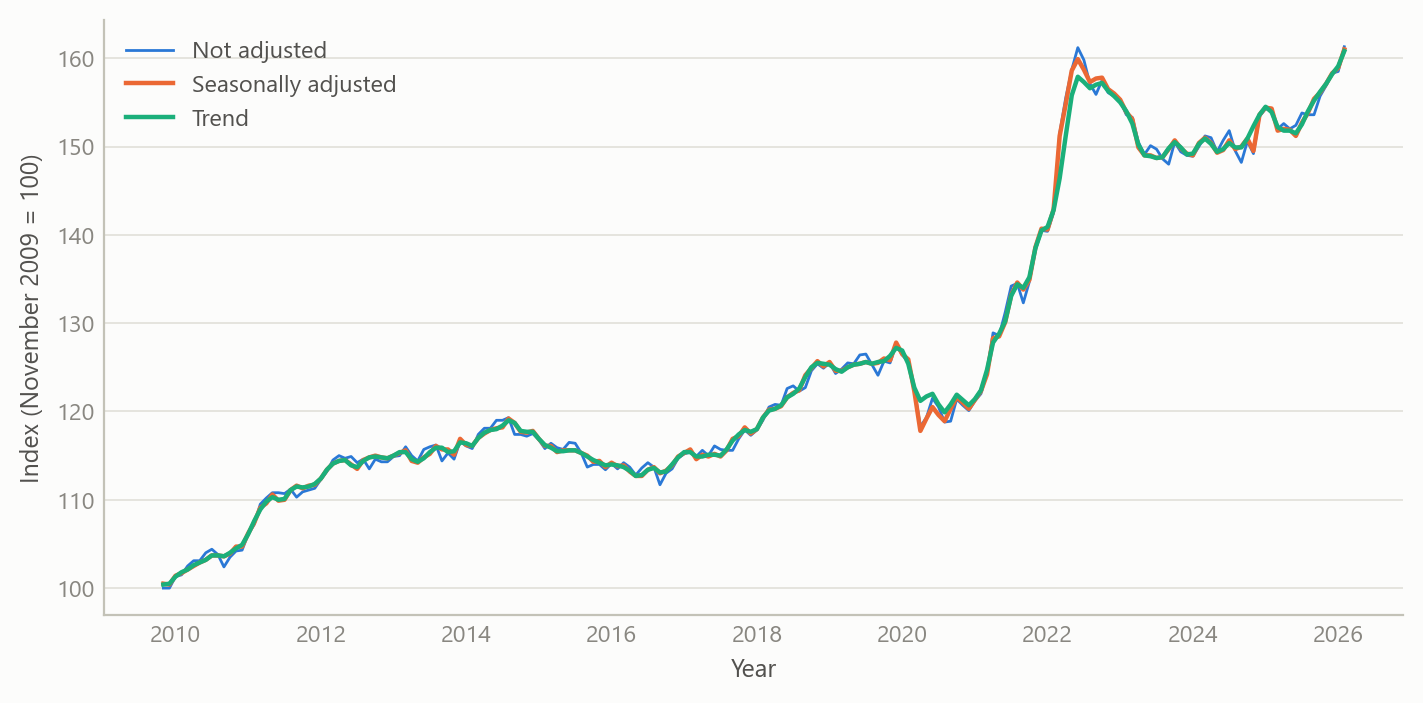
\includegraphics[keepaspectratio]{index_files/figure-latex/fig-decomp-output-1.png}}

}

\caption{\label{fig-decomp}US producer prices for transportation and
warehousing services: not seasonally adjusted, seasonally adjusted, and
the trend from the airline-model decomposition, November 2009 to March
2026. Source: BLS via FRED; the author's decomposition.}

\end{figure}%

\begin{figure}

\centering{

\pandocbounded{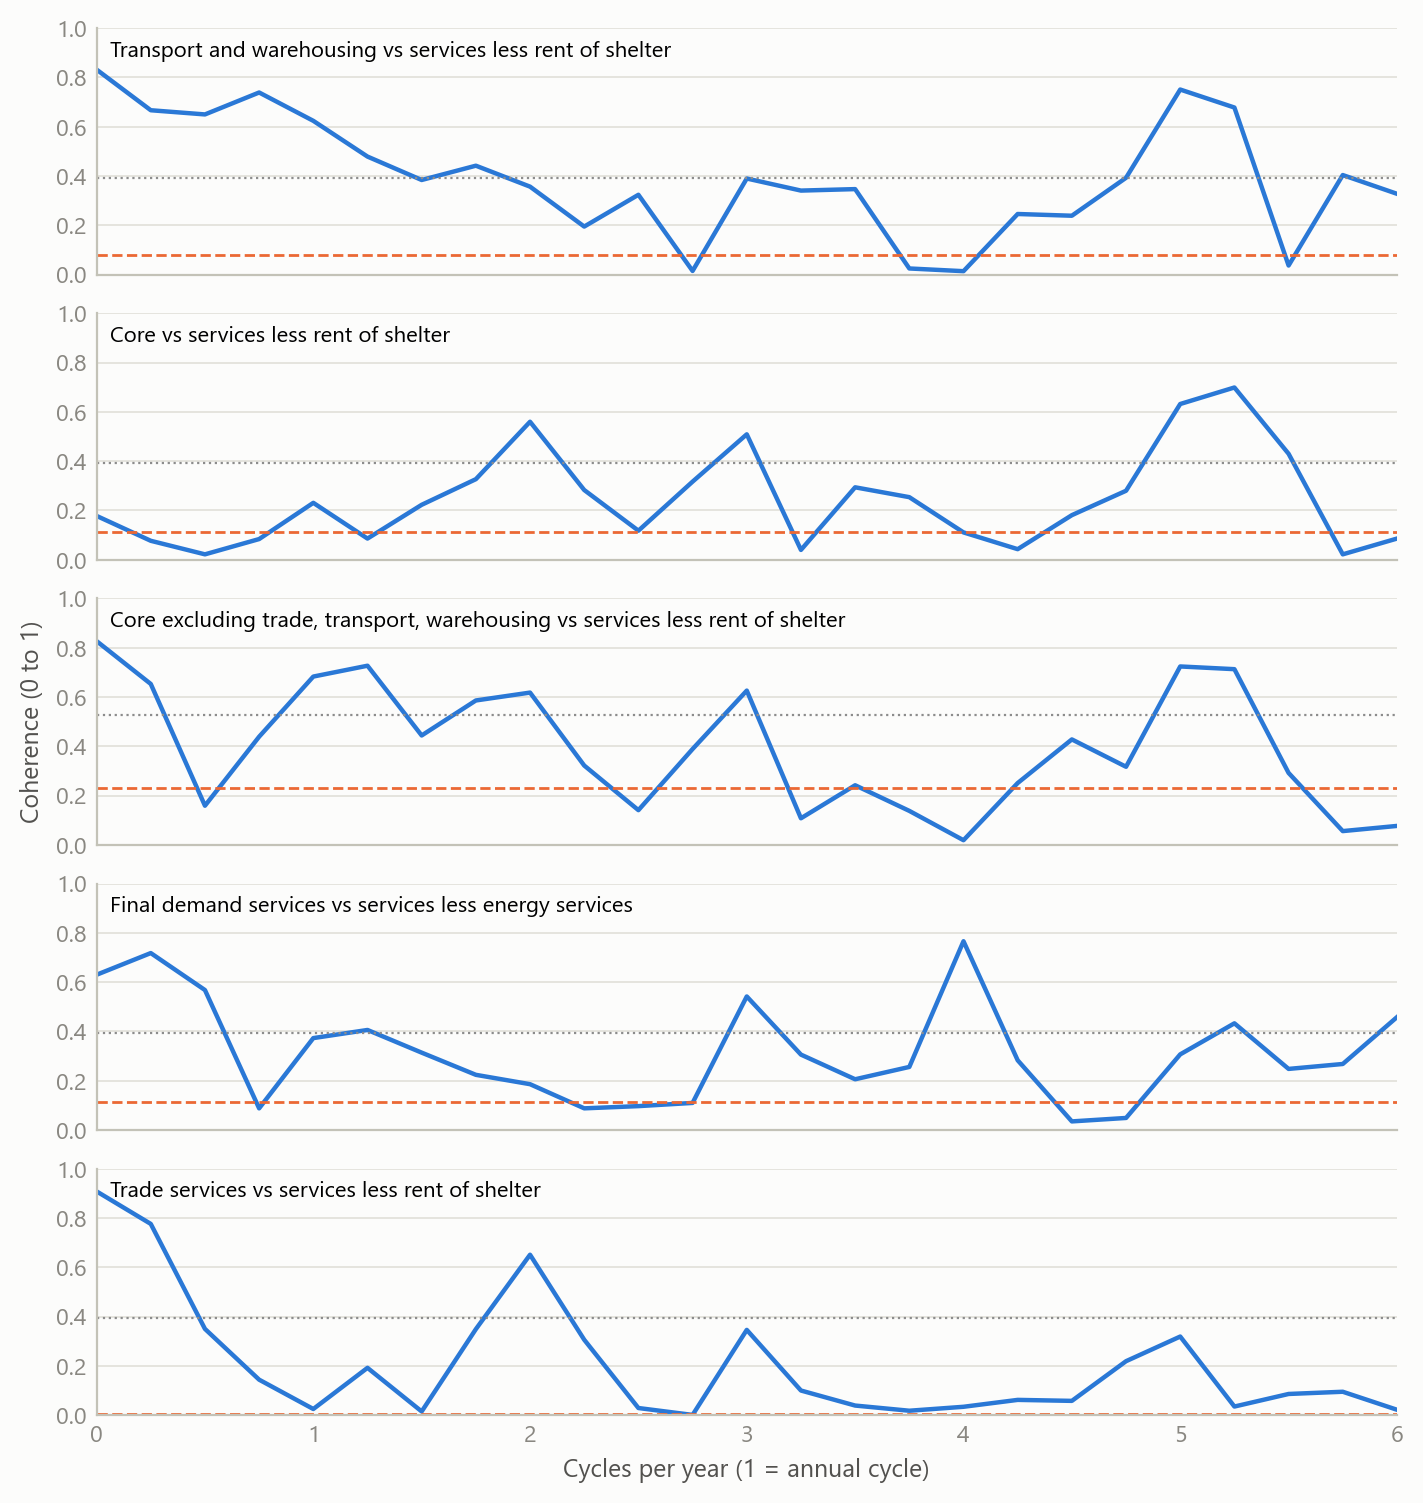
\includegraphics[keepaspectratio]{index_files/figure-latex/fig-coherence-output-1.png}}

}

\caption{\label{fig-coherence}Coherence of monthly log changes for the
five producer-consumer pairs, by cycle length. Dashed: the squared
ordinary correlation. Dotted: the 95\% threshold for coherence under no
relationship. Source: BLS via FRED; the author's calculations.}

\end{figure}%

\begin{figure}

\centering{

\pandocbounded{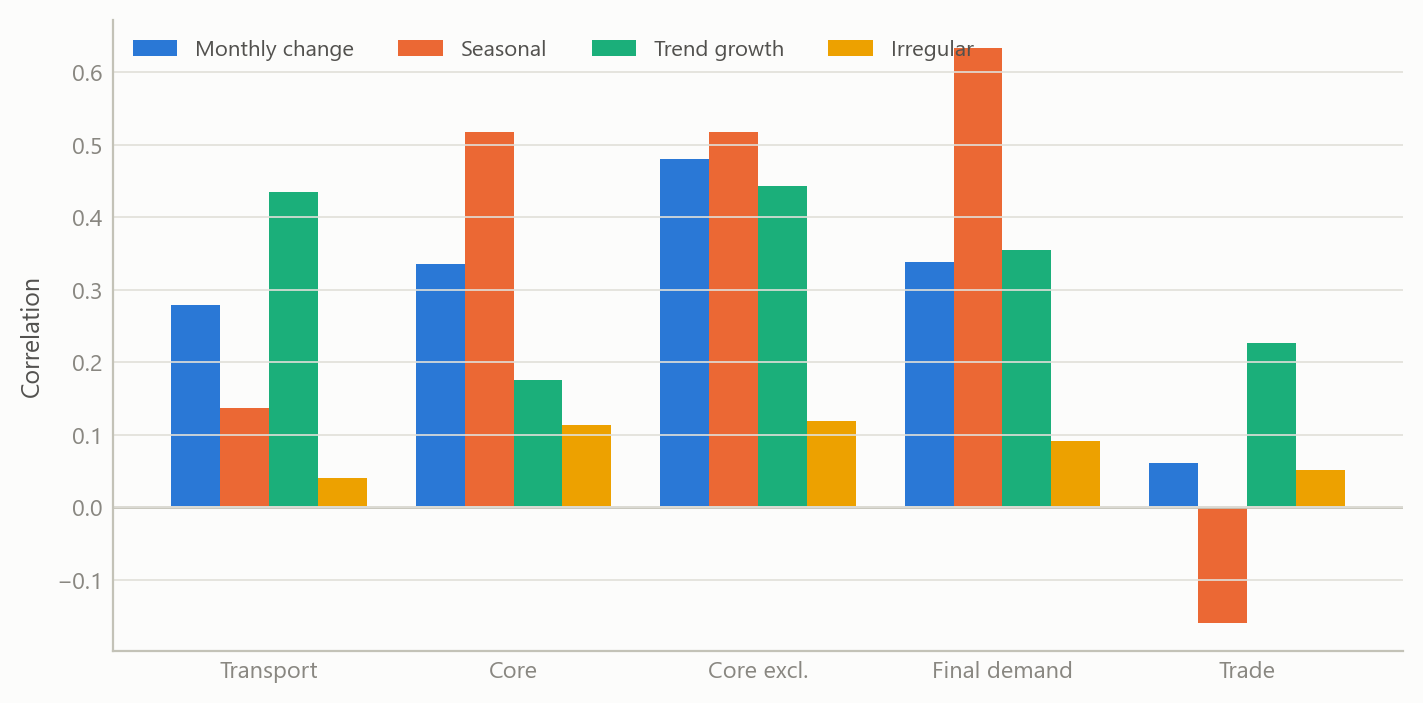
\includegraphics[keepaspectratio]{index_files/figure-latex/fig-components-output-1.png}}

}

\caption{\label{fig-components}Correlation of each producer-consumer
pair, measured on monthly log changes and on each decomposed component.
Source: BLS via FRED; the author's decomposition and calculations.}

\end{figure}%

\begin{figure}

\centering{

\pandocbounded{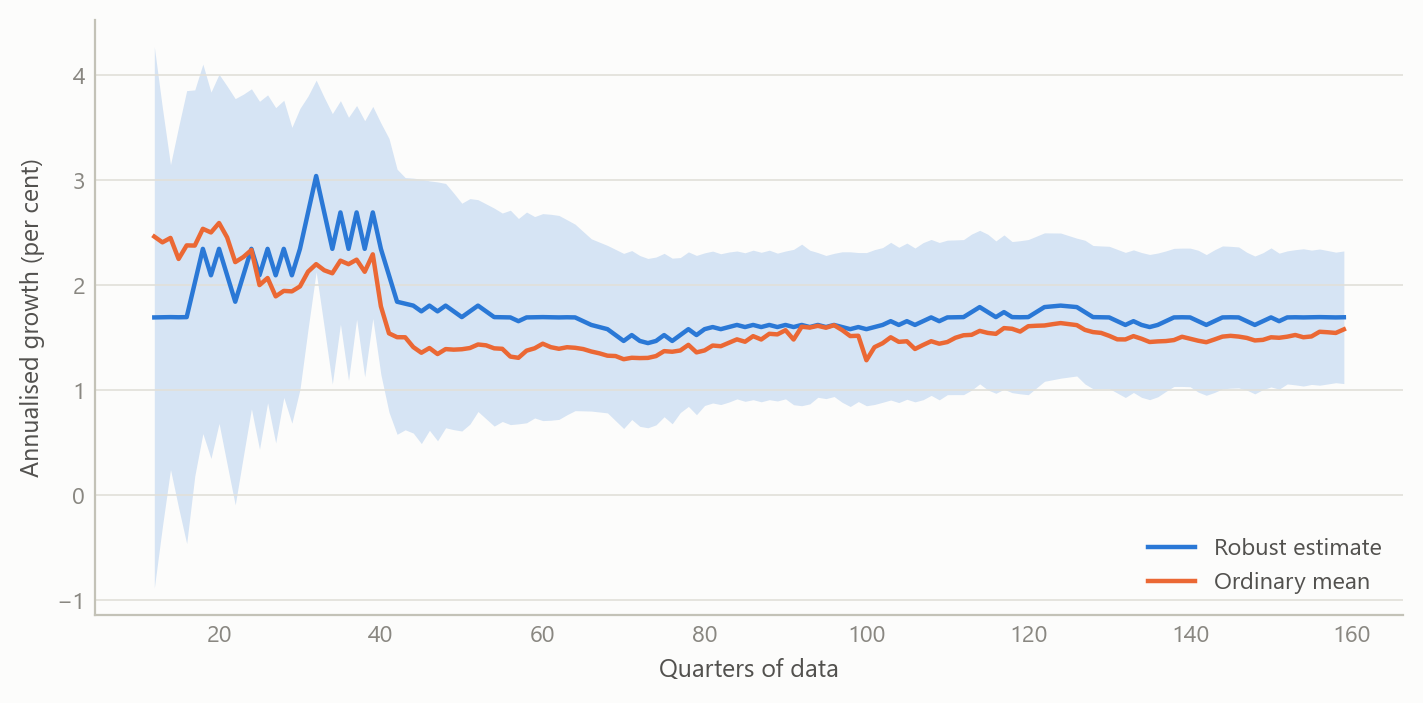
\includegraphics[keepaspectratio]{index_files/figure-latex/fig-steady-output-1.png}}

}

\caption{\label{fig-steady}Long-run growth of a simulated quarterly
series with crisis outliers: the robust estimate against the ordinary
mean, with a 95\% band that tightens as data arrive (simulated data).}

\end{figure}%

\subsection{Insights}\label{insights}

\begin{enumerate}
\def\labelenumi{\arabic{enumi}.}
\tightlist
\item
  \textbf{Decompose before you correlate.} A pair can share a calendar
  and a trend without sharing any short-run dynamics. Splitting the
  series first changes the answer to ``how related are they?''.
\item
  \textbf{Summary statistics average over frequency.} The ordinary
  correlation is a weighted average of coherence across frequencies. A
  relationship that lives at one cycle length is diluted, and a high
  value at the lowest frequency is not evidence of causal pass-through.
\item
  \textbf{Report the transformation.} Log differences and plain
  differences gave correlations up to about 0.05 apart. The effect is
  small, but it is systematic and should be disclosed.
\item
  \textbf{Check the estimator before trusting the peak.} Coherence peaks
  depend on segment length and overlap. Reporting the share of settings
  that remain significant is more honest than quoting the largest value.
\item
  \textbf{Robust growth rates are cheap insurance.} One or two crisis
  quarters can shift an average growth rate by more than its sampling
  error, and a robust estimate with a recursive band shows how much a
  number can be trusted.
\end{enumerate}

\subsection{Limits and next steps}\label{limits-and-next-steps}

The application covers five pairs of US price series, and a refutation
of one claim for those series is not a general statement about price
pass-through. Coherence is not causation: common drivers could produce
coupling in the business-cycle band. The size and variance share of the
frequency-selective link has not been quantified, and the claim that it
has forecasting value has not been tested. The natural next step is a
forecasting experiment in which a band-limited component of producer
prices is used to predict consumer service inflation out of sample,
compared with a naive benchmark. The cross-country long-run growth
estimates also need to be re-run and tabulated before they are shown.

\subsection{About the evidence}\label{about-the-evidence}

The application uses public monthly price series for the United States
from late 2009, about 196 observations per series, and the decomposition
work was applied to US and Mexican price and activity series. The first
three figures are drawn from those public series and the stored
decompositions; the long-run growth figure uses simulated data. The
numbers in the text are the project's own results from the real series.
The work was done from 2025 to 2026, as part of a rebuild of an applied
research toolkit.

Figures and tables marked \emph{simulated} are generated from simulated
data built to share the structure of the analysis (its variables,
horizons and frequencies). They show how the method works and what its
output looks like; they are not the project's results. Results stated in
the text are the project's own. Methods are described at the level of a
methods section. Code and data pipelines are not reproduced here.




\end{document}
